\subsection{Java}

\par Segundo \citeonline{schildt_java_complete_reference}, a primeira versão da linguagem Java foi criada por James Gosling, Patrick Naughton, Chris Warth, Ed Frank e Mike Sheridan na \textit{Sun Microsystems} em 1991 e denominada "Oak" cujo seu principal foco era a interatividade com a TV. Mais tarde, em 1995, a \textit{Sun Mycrosystems} renomeia esta linguagem e anuncia publicamente a tecnologia Java, focando nas aplicações \textit{web}, que em pouco tempo e devido à grande ascensão da internet, cresceu e se mantém em constante evolução até os dias atuais.

\par De acordo com a \citeonline{oracle_about_java_technology}, a tecnologia Java não é apenas uma linguagem, mas também uma plataforma, que teve como modelo uma outra linguagem, o C++ que, por sua vez foi derivada da linguagem C. O C++ e o Java possuem em comum o conceito de orientação a objetos. O que permite a esta linguagem de programação utilizar recursos como: generalização (herança), implementação, polimorfismo, entre outras. Tais funcionalidades permitem ao desenvolvedor escrever códigos reutilizáveis, a fim de facilitar o desenvolvimento do projeto.

Segundo \citeonline{schildt_java_complete_reference}, o recurso denominado generalização (herança) permite ao desenvolvedor criar uma classificação hierárquica de classes. Além disso, é possível escrever uma classe genérica contendo comportamentos comum, e as demais classes, cujo tais comportamentos também serão aplicados a ela, somente precisa generalizar esta classe.

O polimorfismo se refere ao princípio da biologia em que um organismo pode ter diferentes formas ou estados. Este mesmo princípio, também pode ser aplicado à programação orientada a objeto. Desta forma, é possível definir comportamentos que serão compartilhadas entre as classes e suas respectivas sub classes, além de comportamentos próprios cujo apenas as sub classes possuem. Com isto, o comportamento pode ser diferente de acordo com a forma e/ou o estado do objeto \cite{polymorphism_oracle}.

\par Para \citeonline{schildt_java_complete_reference}, o paradigma de orientação a objetos foi criado devido às limitações que o conceito estrutural apresentava quando era utilizado em projetos de grande porte, dificultando o desenvolvimento e manutenção dos mesmos. Este paradigma possibilita ao desenvolvedor aproximar o mundo real ao desenvolvimento de \textit{software}, deixando os objetos do mundo real semelhantes a seus respectivos objetos da computação, possibilitando ao desenvolvedor modelar seus objetos de acordo com suas necessidades \cite{tcc_univas_faria_aspectj_programacao_orientada_aspecto_java}.

\par Retomando a ideia da \citeonline{oracle_about_java_technology}, uma das vantagens da tecnologia Java sob as demais é o fato de ela ser multiplataforma, possibilitando ao desenvolvedor escrever o código apenas uma vez e este, ser executado em qualquer plataforma inclusive em hardwares com menor desempenho. Isto é possível, pois, para executar um programa em Java é necessário possuir uma \textit{Java Virtual Machine} - JVM\footnotemark[12] - instalada no computador. A JVM compreende e executa apenas \textit{bytecodes}\footnotemark[13] e estes por sua vez são obtidos através do processo de compilação do código escrito em Java.

%Nota a respeito da sigla JVM
\footnotetext[12]{JVM: \textit{Java Virtual Machine} - Máquina virtual utilizada pela linguagem Java para execução e compilação de \textit{softwares} desenvolvidos em Java.}

%Nota a respeito de bytecodes
\footnotetext[13]{\textit{Bytecode} é o código interpretado pela JVM. Ele é obtido por meio do processo de compilação de um programa java como mencionado anteriormente.}

\par Todo programa que utiliza Java necessita passar por algumas etapas essenciais. Conforme ilustrado na figura 9, o código é escrito em arquivo de texto com extensão \texttt{.java}, após isto ele será compilado e convertido para um arquivo com extensão \texttt{.class}, cujo o texto é transformado em \textit{bytecodes}. Este arquivo com extensão \texttt{.class} é interpretado pela JVM que é responsável por executar todo o código do programa.

% Imagem do Processo de compilação do Java
\begin{figure}[h!]
	\centerline{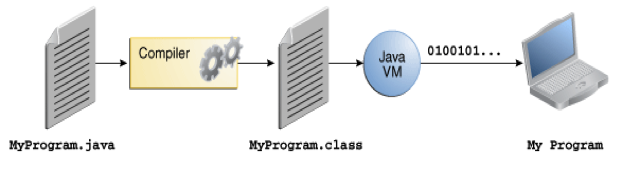
\includegraphics[scale=1]{./imagens/processo_compilacao_java.png}}
	\caption[Uma visão geral do processo de desenvolvimento de software.]
	{Uma visão geral do processo de desenvolvimento de software. \textbf{Fonte:} \citeonline{oracle_about_java_technology}}
	\label{fig:exemplo1}
\end{figure}

\par Por todas as vantagens descritas acima, será empregado o uso desta tecnologia neste projeto.
